% -*- coding: utf-8 -*-
%\documentclass[output=paper]{LSP/langsci} 
\documentclass[output=paper
,newtxmath
,modfonts
,nonflat]{langsci/langscibook} 
% \bibliography{localbibliography} 
% \usepackage{pifont}
\usepackage{savesym}

\savesymbol{downingtriple}
\savesymbol{downingdouble}
\savesymbol{downingquad}
\savesymbol{downingquint}
\savesymbol{suph}
\savesymbol{supj}
\savesymbol{supw}
\savesymbol{sups}
\savesymbol{ts}
\savesymbol{tS}
\savesymbol{devi}
\savesymbol{devu}
\savesymbol{devy}
\savesymbol{deva}
\savesymbol{N}
\savesymbol{Z}
\savesymbol{circled}
\savesymbol{sem}
\savesymbol{row}
\savesymbol{tipa}
\savesymbol{tableauxcounter}
\savesymbol{tabhead}
\savesymbol{inp}
\savesymbol{inpno}
\savesymbol{g}
\savesymbol{hanl}
\savesymbol{hanr}
\savesymbol{kuku}
\savesymbol{ip}
\savesymbol{lipm}
\savesymbol{ripm}
\savesymbol{lipn}
\savesymbol{ripn} 
% \usepackage{amsmath} 
% \usepackage{multicol}
\usepackage{qtree} 
\usepackage{tikz-qtree,tikz-qtree-compat}
% \usepackage{tikz}
\usepackage{upgreek}


%%%%%%%%%%%%%%%%%%%%%%%%%%%%%%%%%%%%%%%%%%%%%%%%%%%%
%%%                                              %%%
%%%           Examples                           %%%
%%%                                              %%%
%%%%%%%%%%%%%%%%%%%%%%%%%%%%%%%%%%%%%%%%%%%%%%%%%%%%
% remove the percentage signs in the following lines
% if your book makes use of linguistic examples
\usepackage{tipa}  
\usepackage{pstricks,pst-xkey,pst-asr}

%for sande et al
\usepackage{pst-jtree}
\usepackage{pst-node}
%\usepackage{savesym}


% \usepackage{subcaption}
\usepackage{multirow}  
\usepackage{./langsci/styles/langsci-optional} 
\usepackage{./langsci/styles/langsci-lgr} 
\usepackage{./langsci/styles/langsci-glyphs} 
\usepackage[normalem]{ulem}
%% if you want the source line of examples to be in italics, uncomment the following line
% \def\exfont{\it}
\usetikzlibrary{arrows.meta,topaths,trees}
\usepackage[linguistics]{forest}
\forestset{
	fairly nice empty nodes/.style={
		delay={where content={}{shape=coordinate,for parent={
					for children={anchor=north}}}{}}
}}
\usepackage{soul}
\usepackage{arydshln}
% \usepackage{subfloat}
\usepackage{langsci/styles/langsci-gb4e} 
   
% \usepackage{linguex}
\usepackage{vowel}

\usepackage{pifont}% http://ctan.org/pkg/pifont
\newcommand{\cmark}{\ding{51}}%
\newcommand{\xmark}{\ding{55}}%
 
 
 %Lamont
 \makeatletter
\g@addto@macro\@floatboxreset\centering
\makeatother

\usepackage{newfloat} 
\DeclareFloatingEnvironment[fileext=tbx,name=Tableau]{tableau}
% %% hyphenation points for line breaks
%% Normally, automatic hyphenation in LaTeX is very good
%% If a word is mis-hyphenated, add it to this file
%%
%% add information to TeX file before \begin{document} with:
%% %% hyphenation points for line breaks
%% Normally, automatic hyphenation in LaTeX is very good
%% If a word is mis-hyphenated, add it to this file
%%
%% add information to TeX file before \begin{document} with:
%% %% hyphenation points for line breaks
%% Normally, automatic hyphenation in LaTeX is very good
%% If a word is mis-hyphenated, add it to this file
%%
%% add information to TeX file before \begin{document} with:
%% \include{localhyphenation}
\hyphenation{
affri-ca-te
affri-ca-tes
com-ple-ments
par-a-digm
Sha-ron
Kings-ton
phe-nom-e-non
Daul-ton
Abu-ba-ka-ri
Ngo-nya-ni
Clem-ents 
King-ston
Tru-cken-brodt
Tab-leau
cophono-logies
mark-edness
Ti-gri-nya
a-mong
Car-stens
Lu-bu-ku-su
}
\hyphenation{
affri-ca-te
affri-ca-tes
com-ple-ments
par-a-digm
Sha-ron
Kings-ton
phe-nom-e-non
Daul-ton
Abu-ba-ka-ri
Ngo-nya-ni
Clem-ents 
King-ston
Tru-cken-brodt
Tab-leau
cophono-logies
mark-edness
Ti-gri-nya
a-mong
Car-stens
Lu-bu-ku-su
}
\hyphenation{
affri-ca-te
affri-ca-tes
com-ple-ments
par-a-digm
Sha-ron
Kings-ton
phe-nom-e-non
Daul-ton
Abu-ba-ka-ri
Ngo-nya-ni
Clem-ents 
King-ston
Tru-cken-brodt
Tab-leau
cophono-logies
mark-edness
Ti-gri-nya
a-mong
Car-stens
Lu-bu-ku-su
}
% %add all your local new commands to this file
\newcommand{\downingquad}[4]{\parbox{2.5cm}{#1}\parbox{3.5cm}{#2}\parbox{2.5cm}{#3}\parbox{3.5cm}{#4}}
\newcommand{\downingtriple}[3]{\parbox{4.5cm}{#1}\parbox{3cm}{#2}\parbox{3cm}{#3}}
\newcommand{\downingdouble}[2]{\parbox{4.5cm}{#1}\parbox{6cm}{#2}}
\newcommand{\downingquint}[5]{\parbox{1.75cm}{#1}\parbox{2.25cm}{#2}\parbox{2cm}{#3}\parbox{3cm}{#4}\parbox{2cm}{#5}}
\newcolumntype{Y}{>{\centering\arraybackslash}X}
\newcolumntype{T}{>{\centering\arraybackslash}m{2cm}}

%commands for Kusmer paper below
\newcommand{\ip}{$\upiota$}
\newcommand{\lipm}{(\_{\ip-Max}}
\newcommand{\ripm}{)\_{\ip-Max}}
\newcommand{\lipn}{(\_{\ip}}
\newcommand{\ripn}{)\_{\ip}}
\renewcommand{\_}[1]{\textsubscript{#1}}


%commands for Pillion paper below
\newcommand{\suph}{\textipa{\super h}}
\newcommand{\supj}{\textipa{\super j}}
\newcommand{\supw}{\textipa{\super w}}
\newcommand{\ts}{\textipa{\t{ts}}}
\newcommand{\tS}{\textipa{\t{tS}}}
\newcommand{\devi}{\textipa{\r*i}}
\newcommand{\devu}{\textipa{\r*u}}
\newcommand{\devy}{\textipa{\r*y}}
\newcommand{\deva}{\textipa{\r*a}}
\renewcommand{\N}{\textipa{N}}
\newcommand{\Z}{\textipa{Z}}
% 

%commands for Diercks paper below
\newcommand{\circled}[1]{\begin{tikzpicture}[baseline=(word.base)]
\node[draw, rounded corners, text height=8pt, text depth=2pt, inner sep=2pt, outer sep=0pt, use as bounding box] (word) {#1};
\end{tikzpicture}
}

%commands for Pesetsky paper below
% \newcommand{\sem}[2][]{\mbox{$[\![ $\textbf{#2}$ ]\!]^{#1}$}}
\newcommand{\sem}[2][]{\mbox{$[[ $\textbf{#2}$ ]]^{#1}$}}

% \newcommand{\ripn}{{\color{red}ripn}}%this is used but never defined. Please update the definition



%commands for Lamont paper below
\newcommand{\row}[4]{
	#1. & 
    /{#2}/ & 
    [{#3}] & 
    `#4' \\ 
}
%\newcounter{tableauxcounter}
\newcommand{\tabhead}[2]{
%     \captionsetup{labelformat=empty}
%     \stepcounter{tableauxcounter}
%     \addtocounter{table}{-1}
% 	\centering
% 	\caption{Tableau \thetableauxcounter: #1}
	\caption{#1}
	\label{#2}
}
\newcommand{\candref}[2]{{(\ref{#1}#2)}}
\newcommand{\tableauref}[1]{{Tableau~\ref{#1}}}
% tableaux
\newcommand{\inp}[1]{\multicolumn{2}{|l||}{{#1}}}
\newcommand{\inpno}[1]{\multicolumn{2}{|l||}{#1}}
\newcommand{\g}{\cellcolor{lightgray}}
\newcommand{\hanl}{\HandLeft}
\newcommand{\hanr}{\HandRight}
\newcommand{\kuku}{Kuk\'{u}}

% \newcommand{\nocaption}[1]{{\color{red} Please provide a caption}}

% \providecommand{\biberror}[1]{{\color{red}#1}}

\definecolor{RED}{cmyk}{0.05,1,0.8,0}


\newfontfamily\amharicfont[Script = Ethiopic, Scale = 1.0]{AbyssinicaSIL}
\newcommand{\amh}[1]{{\amharicfont #1}}

% 
% %Gjersoe
\usepackage{textgreek}
% 
\newcommand{\viol}{\fontfamily{MinionPro-OsF}\selectfont\rotatebox{60}{$\star$}}
\newcommand{\myscalex}{0.45}
\newcommand{\myscaley}{0.65}
%\newcommand{\red}[1]{\textcolor{red}{#1}}
%\newcommand{\blue}[1]{\textcolor{blue}{#1}}
\newcommand{\epen}[1]{\colorbox{jgray}{#1}}
\newcommand{\hand}{{\normalsize \ding{43}}}
\definecolor{jgray}{gray}{0.8} 
\usetikzlibrary{positioning}
\usetikzlibrary{matrix}
\newcommand{\mora}{\textmu\xspace}
\newcommand{\si}{\textsigma\xspace}
\newcommand{\ft}{\textPhi\xspace}
\newcommand{\tone}{\texttau\xspace}
\newcommand{\word}{\textomega\xspace}
% \newcommand{\ts}{\texttslig}
\newcommand{\fns}{\footnotesize}
\newcommand{\ns}{\normalsize}
\newcommand{\vs}{\vspace{1em}}
\newcommand{\bs}{\textbackslash}   % backslash
\newcommand{\cmd}[1]{{\bf \color{red}#1}}   % highlights command
\newcommand{\scell}[2][l]{\begin{tabular}[#1]{@{}c@{}}#2\end{tabular}}
% \interfootnotelinepenalty=10000

% --- Snider Representations --- %

\newcommand{\RepLevelHh}{
\begin{minipage}{0.10\textwidth}
\begin{tikzpicture}[xscale=\myscalex,yscale=\myscaley]
%\node (syl) at (0,0) {Hi};
\node (Rt) at (0,1) {o};
\node (H) at (-0.5,2) {H};
\node (R) at (0.5,3) {h};
%\draw [thick] (syl.north) -- (Rt.south) ;
\draw [thick] (Rt.north) -- (H.south) ;
\draw [thick] (Rt.north) -- (R.south) ;
\end{tikzpicture}
\end{minipage}
}

\newcommand{\RepLevelLh}{
\begin{minipage}{0.10\textwidth}
\begin{tikzpicture}[xscale=\myscalex,yscale=\myscaley]
%\node (syl) at (0,0) {Mid2};
\node (Rt) at (0,1) {o};
\node (H) at (-0.5,2) {L};
\node (R) at (0.5,3) {h};
%\draw [thick] (syl.north) -- (Rt.south) ;
\draw [thick] (Rt.north) -- (H.south) ;
\draw [thick] (Rt.north) -- (R.south) ;
\end{tikzpicture}
\end{minipage}
}

\newcommand{\RepLevelHl}{
\begin{minipage}{0.10\textwidth}
\begin{tikzpicture}[xscale=\myscalex,yscale=\myscaley]
%\node (syl) at (0,0) {Mid1};
\node (Rt) at (0,1) {o};
\node (H) at (-0.5,2) {H};
\node (R) at (0.5,3) {l};
%\draw [thick] (syl.north) -- (Rt.south) ;
\draw [thick] (Rt.north) -- (H.south) ;
\draw [thick] (Rt.north) -- (R.south) ;
\end{tikzpicture}
\end{minipage}
}

\newcommand{\RepLevelLl}{
\begin{minipage}{0.10\textwidth}
\begin{tikzpicture}[xscale=\myscalex,yscale=\myscaley]
%\node (syl) at (0,0) {Lo};
\node (Rt) at (0,1) {o};
\node (H) at (-0.5,2) {L};
\node (R) at (0.5,3) {l};
%\draw [thick] (syl.north) -- (Rt.south) ;
\draw [thick] (Rt.north) -- (H.south) ;
\draw [thick] (Rt.north) -- (R.south) ;
\end{tikzpicture}
\end{minipage}
}

% --- Representations --- %

\newcommand{\RepLevel}{
\begin{minipage}{0.10\textwidth}
\begin{tikzpicture}[xscale=\myscalex,yscale=\myscaley]
\node (syl) at (0,0) {\textsigma};
\node (Rt) at (0,1) {o};
\node (H) at (-0.5,2) {\texttau};
\node (R) at (0.5,3) {\textrho};
\draw [thick] (syl.north) -- (Rt.south) ;
\draw [thick] (Rt.north) -- (H.south) ;
\draw [thick] (Rt.north) -- (R.south) ;
\end{tikzpicture}
\end{minipage}
}

\newcommand{\RepContour}{
\begin{minipage}{0.10\textwidth}
\begin{tikzpicture}[xscale=\myscalex,yscale=\myscaley]
\node (syl) at (0,0) {\textsigma};
\node (Rt) at (0,1) {o};
\node (H) at (-0.5,2) {\texttau};
\node (R) at (0.5,3) {\textrho};
\node (Rt2) at (1.5,1.0) {o};
%\node (H2) at (1.0,2) {$\tau$};
%\node (R2) at (2.0,2.5) {R};
\draw [thick] (syl.north) -- (Rt.south) ;
\draw [thick] (Rt.north) -- (H.south) ;
\draw [thick] (Rt.north) -- (R.south) ;
\draw [thick] (syl.north) -- (Rt2.south) ;
%\draw [thick] (Rt2.north) -- (H2.south) ;
%\draw [thick] (Rt2.north) -- (R2.south) ;
\end{tikzpicture}
\end{minipage}
}


% --- OT constraints --- %

\newcommand{\IllustrationDown}{
\begin{minipage}{0.09\textwidth}
\begin{tikzpicture}[xscale=0.7,yscale=0.45]
\node (reg) at (0,0.75) {{\small \textalpha}};
\node (arrow) at (0,0) {{\fns $\downarrow$}};
\node (Rt) at (0,-0.75) {{\small \textbeta}};
\end{tikzpicture}
\end{minipage}
}

\newcommand{\IllustrationUp}{
\begin{minipage}{0.09\textwidth}
\begin{tikzpicture}[xscale=0.7,yscale=0.45]
\node (reg) at (0,0.75) {{\small \textalpha}};
\node (arrow) at (0,0) {{\fns $\uparrow$}};
\node (Rt) at (0,-0.75) {{\small \textbeta}};
\end{tikzpicture}
\end{minipage}
}

\newcommand{\MaxAB}{
\begin{minipage}{0.09\textwidth}
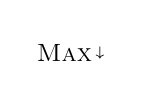
\begin{tikzpicture}[xscale=0.6,yscale=0.4]
\node (max) at (0,0) {{\small \textsc{Max}}};
\node (reg) at (0.75,0.5) {{\fns \textalpha}};
\node (arrow) at (0.75,0) {{\tiny $\downarrow$}};
\node (Rt) at (0.75,-0.5) {{\fns \textbeta}};
\end{tikzpicture}
\end{minipage}
}

\newcommand{\DepAB}{
\begin{minipage}{0.09\textwidth}
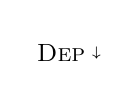
\begin{tikzpicture}[xscale=0.6,yscale=0.4]
\node (max) at (0,0) {{\small \textsc{Dep}}};
\node (reg) at (0.75,0.5) {{\fns \textalpha}};
\node (arrow) at (0.75,0) {{\tiny $\downarrow$}};
\node (Rt) at (0.75,-0.5) {{\fns \textbeta}};
\end{tikzpicture}
\end{minipage}
}

\newcommand{\DepHReg}{
\begin{minipage}{0.055\textwidth}
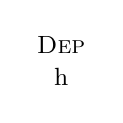
\begin{tikzpicture}[xscale=0.6,yscale=0.4]
\node (dep) at (0,0) {{\small \textsc{Dep}}};
\node (reg) at (0,-1.0) {{\small h}};
\end{tikzpicture}
\end{minipage}
}

\newcommand{\DepLReg}{
\begin{minipage}{0.055\textwidth}
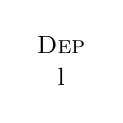
\begin{tikzpicture}[xscale=0.6,yscale=0.4]
\node (dep) at (0,0) {{\small \textsc{Dep}}};
\node (reg) at (0,-1.0) {{\small l}};
\end{tikzpicture}
\end{minipage}
}

\newcommand{\DepReg}{
\begin{minipage}{0.055\textwidth}
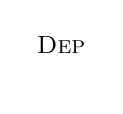
\begin{tikzpicture}[xscale=0.6,yscale=0.4]
\node (dep) at (0,0) {{\small \textsc{Dep}}};
\node (reg) at (0,-1.0) {{\small \textrho}};
\end{tikzpicture}
\end{minipage}
}

\newcommand{\DepTRt}{
\begin{minipage}{0.1\textwidth}
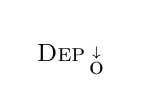
\begin{tikzpicture}[xscale=0.6,yscale=0.4]
\node (dep) at (0,0) {{\small \textsc{Dep}}};
\node (t) at (0.75,0.5) {{\fns \texttau}};
\node (arrow) at (0.75,0) {{\tiny $\downarrow$}};
\node (Rt) at (0.75,-0.5) {{\fns o}};
\end{tikzpicture}
\end{minipage}
}

\newcommand{\MaxRegRt}{
\begin{minipage}{0.1\textwidth}
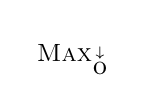
\begin{tikzpicture}[xscale=0.6,yscale=0.4]
\node (max) at (0,0) {{\small \textsc{Max}}};
\node (arrow) at (0.75,0) {{\tiny $\downarrow$}};
\node (Rt) at (0.75,-0.5) {{\fns o}};
\node (reg) at (0.75,0.5) {{\fns \textrho}};
\end{tikzpicture}
\end{minipage}
}

\newcommand{\RegToneByRt}{
\begin{minipage}{0.06\textwidth}
\begin{tikzpicture}[xscale=0.6,yscale=0.5]
\node[rotate=20] (arrow1) at (-0.15,0) {{\fns $\uparrow$}};
\node[rotate=340] (arrow2) at (0.15,0) {{\fns $\uparrow$}};
\node (Rt) at (0,-0.55) {{\small o}};
\node (reg) at (0.4,0.55) {{\small \textrho}};
\node (tone) at (-0.4,0.55) {{\small \texttau}};
\end{tikzpicture}
\end{minipage}
}

\newcommand{\RegToneBySyl}{
\begin{minipage}{0.06\textwidth}
\begin{tikzpicture}[xscale=0.6,yscale=0.5]
\node[rotate=20] (arrow1) at (-0.15,0) {{\fns $\uparrow$}};
\node[rotate=340] (arrow2) at (0.15,0) {{\fns $\uparrow$}};
\node (Rt) at (0,-0.55) {{\small \textsigma}};
\node (reg) at (0.4,0.55) {{\small \textrho}};
\node (tone) at (-0.4,0.55) {{\small \texttau}};
\end{tikzpicture}
\end{minipage}
}

\newcommand{\DepTone}{
\begin{minipage}{0.055\textwidth}
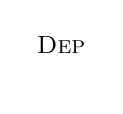
\begin{tikzpicture}[xscale=0.6,yscale=0.4]
\node (dep) at (0,0) {{\small \textsc{Dep}}};
\node (tone) at (0,-1.0) {{\small \texttau}};
\end{tikzpicture}
\end{minipage}
}

\newcommand{\DepTonalRt}{
\begin{minipage}{0.055\textwidth}
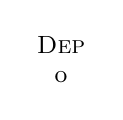
\begin{tikzpicture}[xscale=0.6,yscale=0.4]
\node (dep) at (0,0) {{\small \textsc{Dep}}};
\node (tone) at (0,-1.0) {{\small o}};
\end{tikzpicture}
\end{minipage}
}

\newcommand{\DepL}{
\begin{minipage}{0.055\textwidth}
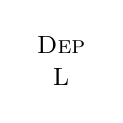
\begin{tikzpicture}[xscale=0.6,yscale=0.4]
\node (dep) at (0,0) {{\small \textsc{Dep}}};
\node (tone) at (0,-1.0) {{\small L}};
\end{tikzpicture}
\end{minipage}
}

\newcommand{\DepH}{
\begin{minipage}{0.055\textwidth}
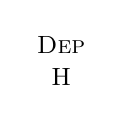
\begin{tikzpicture}[xscale=0.6,yscale=0.4]
\node (dep) at (0,0) {{\small \textsc{Dep}}};
\node (tone) at (0,-1.0) {{\small H}};
\end{tikzpicture}
\end{minipage}
}

\newcommand{\NoMultDiff}{{\small *loh}}
\newcommand{\Alt}{{\small \textsc{Alt}}}
\newcommand{\NoSkip}{{\small \scell{\textsc{No}\\\textsc{Skip}}}}


\newcommand{\RegDomRt}{
\begin{minipage}{0.030\textwidth}
\begin{tikzpicture}[xscale=0.6,yscale=0.5]
\node (arrow) at (0,0) {{\fns $\downarrow$}};
\node (Rt) at (0,-0.55) {{\small o}};
\node (reg) at (0,0.55) {{\small \textrho}};
\end{tikzpicture}
\end{minipage}
}

\newcommand{\DepRegRt}{
\begin{minipage}{0.1\textwidth}
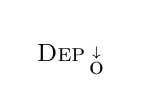
\begin{tikzpicture}[xscale=0.6,yscale=0.4]
\node (dep) at (0,0) {{\small \textsc{Dep}}};
\node (arrow) at (0.75,0) {{\tiny $\downarrow$}};
\node (Rt) at (0.75,-0.5) {{\fns o}};
\node (reg) at (0.75,0.5) {{\fns \textrho}};
\end{tikzpicture}
\end{minipage}
}

% unused

\newcommand{\ToneByRt}{
\begin{minipage}{0.05\textwidth}
\begin{tikzpicture}[xscale=0.6,yscale=0.5]
\node (arrow) at (0,0) {{\fns $\uparrow$}};
\node (Rt) at (0,-0.55) {{\small o}};
\node (tone) at (0,0.55) {{\small \texttau}};
\end{tikzpicture}
\end{minipage}
}

\newcommand{\RegByRt}{
\begin{minipage}{0.05\textwidth}
\begin{tikzpicture}[xscale=0.6,yscale=0.5]
\node (arrow) at (0,0) {{\fns $\uparrow$}};
\node (Rt) at (0,-0.55) {{\small o}};
\node (reg) at (0,0.55) {{\small \textrho}};
\end{tikzpicture}
\end{minipage}
}

\newcommand{\ToneDomRt}{
\begin{minipage}{0.05\textwidth}
\begin{tikzpicture}[xscale=0.6,yscale=0.5]
\node (arrow) at (0,0) {{\fns $\downarrow$}};
\node (Rt) at (0,-0.55) {{\small o}};
\node (tone) at (0,0.55) {{\small \texttau}};
\end{tikzpicture}
\end{minipage}
}

% --- OT tableaus --- %

% Sec. 3.2, first tabl.

\newcommand{\OTHLInput}{
\begin{minipage}{0.17\textwidth}
\begin{tikzpicture}[xscale=\myscalex,yscale=\myscaley]
\node (tone) at (2,0) {(= H)};
\node (syl) at (0,0) {\textsigma};
\node (Rt) at (0,1) {o};
\node (H) at (-0.5,2) {H};
\node (R) at (0.5,3) {h};
\node (Rt2) at (1.5,1.0) {o};
%\node (H2) at (1.0,2) {\epen{L}};
\node (R2) at (2.0,3) {\blue{l}};
\draw [thick] (syl.north) -- (Rt.south) ;
\draw [thick] (Rt.north) -- (H.south) ;
\draw [thick] (Rt.north) -- (R.south) ;
\draw [thick] (syl.north) -- (Rt2.south) ;
%\draw [dashed] (Rt2.north) -- (H2.south) ;
%\draw [dashed] (Rt2.north) -- (R2.south) ;
\end{tikzpicture}
\end{minipage}
}

\newcommand{\OTHLWinner}{
\begin{minipage}{0.17\textwidth}
\begin{tikzpicture}[xscale=\myscalex,yscale=\myscaley]
\node (tone) at (2,0) {(= HL)};
\node (syl) at (0,0) {\textsigma};
\node (Rt) at (0,1) {o};
\node (H) at (-0.5,2) {H};
\node (R) at (0.5,3) {h};
\node (Rt2) at (1.5,1.0) {o};
\node (H2) at (1.0,2) {\epen{L}};
\node (R2) at (2.0,3) {\blue{l}};
\draw [thick] (syl.north) -- (Rt.south) ;
\draw [thick] (Rt.north) -- (H.south) ;
\draw [thick] (Rt.north) -- (R.south) ;
\draw [thick] (syl.north) -- (Rt2.south) ;
\draw [dashed] (Rt2.north) -- (H2.south) ;
\draw [dashed] (Rt2.north) -- (R2.south) ;
\end{tikzpicture}
\end{minipage}
}

\newcommand{\OTHLSpreadingHOnly}{
\begin{minipage}{0.17\textwidth}
\begin{tikzpicture}[xscale=\myscalex,yscale=\myscaley]
\node (tone) at (2,0) {(= HM)};
\node (syl) at (0,0) {\textsigma};
\node (Rt) at (0,1) {o};
\node (H) at (-0.5,2) {H};
\node (R) at (0.5,3) {h};
\node (Rt2) at (1.5,1.0) {o};
%\node (H2) at (1.0,2) {\epen{L}};
\node (R2) at (2.0,3) {\blue{l}};
\draw [thick] (syl.north) -- (Rt.south) ;
\draw [thick] (Rt.north) -- (H.south) ;
\draw [thick] (Rt.north) -- (R.south) ;
\draw [thick] (syl.north) -- (Rt2.south) ;
\draw [dashed] (Rt2.north) -- (R2.south) ;
\draw [dashed] (Rt2.north) -- (H.south) ;
\end{tikzpicture}
\end{minipage}
}

\newcommand{\OTHLInsertH}{
\begin{minipage}{0.17\textwidth}
\begin{tikzpicture}[xscale=\myscalex,yscale=\myscaley]
\node (tone) at (2,0) {(= HM)};
\node (syl) at (0,0) {\textsigma};
\node (Rt) at (0,1) {o};
\node (H) at (-0.5,2) {H};
\node (R) at (0.5,3) {h};
\node (Rt2) at (1.5,1.0) {o};
\node (H2) at (1.0,2) {\epen{H}};
\node (R2) at (2.0,3) {\blue{l}};
\draw [thick] (syl.north) -- (Rt.south) ;
\draw [thick] (Rt.north) -- (H.south) ;
\draw [thick] (Rt.north) -- (R.south) ;
\draw [thick] (syl.north) -- (Rt2.south) ;
\draw [dashed] (Rt2.north) -- (H2.south) ;
\draw [dashed] (Rt2.north) -- (R2.south) ;
\end{tikzpicture}
\end{minipage}
}

\newcommand{\OTHLOverwriting}{
\begin{minipage}{0.17\textwidth}
\begin{tikzpicture}[xscale=\myscalex,yscale=\myscaley]
\node (syl) at (0,0) {\textsigma};
\node (Rt) at (0,1) {o};
\node (H) at (-0.5,2) {H};
\node (R) at (0.5,3) {h};
\node (Rt2) at (1.5,1.0) {o};
%\node (H2) at (1.0,2) {\epen{L}};
\node (R2) at (2.0,3) {\blue{l}};
\draw [thick] (syl.north) -- (Rt.south) ;
\draw [thick] (Rt.north) -- (H.south) ;
\draw [thick] (Rt.north) -- (R.south) ;
\draw [thick] (syl.north) -- (Rt2.south) ;
%\draw [dashed] (Rt2.north) -- (H2.south) ;
\draw [dashed] (Rt.north) -- (R2.south) ;
\node (del) at (0.3,1.9) {\textbf{=}};
\end{tikzpicture}
\end{minipage}
}

\newcommand{\OTHLSpreading}{
\begin{minipage}{0.17\textwidth}
\begin{tikzpicture}[xscale=\myscalex,yscale=\myscaley]
\node (syl) at (0,0) {\textsigma};
\node (Rt) at (0,1) {o};
\node (H) at (-0.5,2) {H};
\node (R) at (0.5,3) {h};
\node (Rt2) at (1.5,1.0) {o};
%\node (H2) at (1.0,2) {\epen{L}};
\node (R2) at (2.0,3) {\blue{l}};
\draw [thick] (syl.north) -- (Rt.south) ;
\draw [thick] (Rt.north) -- (H.south) ;
\draw [thick] (Rt.north) -- (R.south) ;
\draw [thick] (syl.north) -- (Rt2.south) ;
%\draw [dashed] (Rt2.north) -- (H2.south) ;
\draw [dashed] (Rt2.north) -- (H.south) ;
\draw [dashed] (Rt2.north) -- (R.south) ;
\end{tikzpicture}
\end{minipage}
}

% Sec. 4.2, second tabl.: phrase-medial position

\newcommand{\OTHnoLInput}{
\begin{minipage}{0.17\textwidth}
\begin{tikzpicture}[xscale=\myscalex,yscale=\myscaley]
\node (tone) at (2,0) {(= H)};
\node (syl) at (0,0) {\textsigma};
\node (Rt) at (0,1) {o};
\node (H) at (-0.5,2) {H};
\node (R) at (0.5,3) {h};
\node (Rt2) at (1.5,1.0) {o};
%\node (H2) at (1.0,2) {\epen{L}};
%\node (R2) at (2.0,3) {\blue{l}};
\draw [thick] (syl.north) -- (Rt.south) ;
\draw [thick] (Rt.north) -- (H.south) ;
\draw [thick] (Rt.north) -- (R.south) ;
\draw [thick] (syl.north) -- (Rt2.south) ;
\end{tikzpicture}
\end{minipage}
}

\newcommand{\OTHnoLEpenth}{
\begin{minipage}{0.17\textwidth}
\begin{tikzpicture}[xscale=\myscalex,yscale=\myscaley]
\node (tone) at (2,0) {(= HM)};
\node (syl) at (0,0) {\textsigma};
\node (Rt) at (0,1) {o};
\node (H) at (-0.5,2) {H};
\node (R) at (0.5,3) {h};
\node (Rt2) at (1.5,1.0) {o};
\node (H2) at (1.0,2) {\epen{L}};
\node (R2) at (2.0,3) {\epen{h}};
\draw [thick] (syl.north) -- (Rt.south) ;
\draw [thick] (Rt.north) -- (H.south) ;
\draw [thick] (Rt.north) -- (R.south) ;
\draw [thick] (syl.north) -- (Rt2.south) ;
\draw [dashed] (Rt2.north) -- (H2.south) ;
\draw [dashed] (Rt2.north) -- (R2.south) ;
\end{tikzpicture}
\end{minipage}
}

\newcommand{\OTHnoLSpreading}{
\begin{minipage}{0.17\textwidth}
\begin{tikzpicture}[xscale=\myscalex,yscale=\myscaley]
\node (tone) at (2,0) {(= HH)};
\node (syl) at (0,0) {\textsigma};
\node (Rt) at (0,1) {o};
\node (H) at (-0.5,2) {H};
\node (R) at (0.5,3) {h};
\node (Rt2) at (1.5,1.0) {o};
%\node (H2) at (1.0,2) {\epen{L}};
%\node (R2) at (2.0,3) {\blue{l}};
\draw [thick] (syl.north) -- (Rt.south) ;
\draw [thick] (Rt.north) -- (H.south) ;
\draw [thick] (Rt.north) -- (R.south) ;
\draw [thick] (syl.north) -- (Rt2.south) ;
\draw [dashed] (Rt2.north) -- (H.south) ;
\draw [dashed] (Rt2.north) -- (R.south) ;
\end{tikzpicture}
\end{minipage}
}

% Sec. 4.2, third tabl., LM is unaffected by L\%

\newcommand{\OTLMInput}{
\begin{minipage}{0.2\textwidth}
\begin{tikzpicture}[xscale=\myscalex,yscale=\myscaley]
\node (tone) at (2,0) {(= LM)};
\node (syl) at (0,0) {\textsigma};
\node (Rt) at (0,1) {o};
\node (H) at (-0.5,2) {L};
\node (R) at (0.5,3) {l};
\node (Rt2) at (1.5,1.0) {o};
\node (H2) at (1.0,2) {L};
\node (R2) at (2.0,3) {h};
\node (R3) at (3.0,3) {\blue{l}};
\draw [thick] (syl.north) -- (Rt.south) ;
\draw [thick] (Rt.north) -- (H.south) ;
\draw [thick] (Rt.north) -- (R.south) ;
\draw [thick] (syl.north) -- (Rt2.south) ;
\draw [thick] (Rt2.north) -- (H2.south) ;
\draw [thick] (Rt2.north) -- (R2.south) ;
\end{tikzpicture}
\end{minipage}
}

\newcommand{\OTLMReplace}{
\begin{minipage}{0.2\textwidth}
\begin{tikzpicture}[xscale=\myscalex,yscale=\myscaley]
\node (tone) at (2,0) {(= LL)};
\node (syl) at (0,0) {\textsigma};
\node (Rt) at (0,1) {o};
\node (H) at (-0.5,2) {L};
\node (R) at (0.5,3) {l};
\node (Rt2) at (1.5,1.0) {o};
\node (H2) at (1.0,2) {L};
\node (R2) at (2.0,3) {h};
\node (R3) at (3.0,3) {\blue{l}};
\draw [thick] (syl.north) -- (Rt.south) ;
\draw [thick] (Rt.north) -- (H.south) ;
\draw [thick] (Rt.north) -- (R.south) ;
\draw [thick] (syl.north) -- (Rt2.south) ;
\draw [thick] (Rt2.north) -- (H2.south) ;
\draw [thick] (Rt2.north) -- (R2.south) ;
\draw [dashed] (Rt2.north) -- (R3.south) ;
\node (del) at (1.8,2.1) {\textbf{=}};
\end{tikzpicture}
\end{minipage}
}

\newcommand{\OTLMTwoReg}{
\begin{minipage}{0.2\textwidth}
\begin{tikzpicture}[xscale=\myscalex,yscale=\myscaley]
\node (tone) at (2,0) {(= LML)};
\node (syl) at (0,0) {\textsigma};
\node (Rt) at (0,1) {o};
\node (H) at (-0.5,2) {L};
\node (R) at (0.5,3) {l};
\node (Rt2) at (1.5,1.0) {o};
\node (H2) at (1.0,2) {L};
\node (R2) at (2.0,3) {h};
\node (R3) at (3.0,3) {\blue{l}};
\draw [thick] (syl.north) -- (Rt.south) ;
\draw [thick] (Rt.north) -- (H.south) ;
\draw [thick] (Rt.north) -- (R.south) ;
\draw [thick] (syl.north) -- (Rt2.south) ;
\draw [thick] (Rt2.north) -- (H2.south) ;
\draw [thick] (Rt2.north) -- (R2.south) ;
\draw [dashed] (Rt2.north) -- (R3.south) ;
\end{tikzpicture}
\end{minipage}
}

% Sec. 4.2, fourth tabl., L is affected by L\% but M is not

\newcommand{\OTLInput}{
\begin{minipage}{0.17\textwidth}
\begin{tikzpicture}[xscale=\myscalex,yscale=\myscaley]
\node (tone) at (2,0) {(= L)};
\node (syl) at (0,0) {\textsigma};
\node (Rt) at (0,1) {o};
\node (H) at (-0.5,2) {L};
\node (R) at (0.5,3) {l};
\node (R2) at (2,3) {\blue{l}};
\draw [thick] (syl.north) -- (Rt.south) ;
\draw [thick] (Rt.north) -- (H.south) ;
\draw [thick] (Rt.north) -- (R.south) ;
\end{tikzpicture}
\end{minipage}
}

\newcommand{\OTLLowered}{
\begin{minipage}{0.17\textwidth}
\begin{tikzpicture}[xscale=\myscalex,yscale=\myscaley]
\node (tone) at (2,0) {(= LL)};
\node (syl) at (0,0) {\textsigma};
\node (Rt) at (0,1) {o};
\node (H) at (-0.5,2) {L};
\node (R) at (0.5,3) {l};
\node (R2) at (2,3) {\blue{l}};
\draw [thick] (syl.north) -- (Rt.south) ;
\draw [thick] (Rt.north) -- (H.south) ;
\draw [thick] (Rt.north) -- (R.south) ;
\draw [dashed] (Rt.north) -- (R2.south) ;
\end{tikzpicture}
\end{minipage}
}

\newcommand{\OTMInput}{
\begin{minipage}{0.17\textwidth}
\begin{tikzpicture}[xscale=\myscalex,yscale=\myscaley]
\node (tone) at (2,0) {(= M)};
\node (syl) at (0,0) {\textsigma};
\node (Rt) at (0,1) {o};
\node (H) at (-0.5,2) {L};
\node (R) at (0.5,3) {h};
\node (R2) at (2,3) {\blue{l}};
\draw [thick] (syl.north) -- (Rt.south) ;
\draw [thick] (Rt.north) -- (H.south) ;
\draw [thick] (Rt.north) -- (R.south) ;
\end{tikzpicture}
\end{minipage}
}

\newcommand{\OTMLowered}{
\begin{minipage}{0.17\textwidth}
\begin{tikzpicture}[xscale=\myscalex,yscale=\myscaley]
\node (tone) at (2,0) {(= ML)};
\node (syl) at (0,0) {\textsigma};
\node (Rt) at (0,1) {o};
\node (H) at (-0.5,2) {L};
\node (R) at (0.5,3) {h};
\node (R2) at (2,3) {\blue{l}};
\draw [thick] (syl.north) -- (Rt.south) ;
\draw [thick] (Rt.north) -- (H.south) ;
\draw [thick] (Rt.north) -- (R.south) ;
\draw [dashed] (Rt.north) -- (R2.south) ;
\end{tikzpicture}
\end{minipage}
}

% Sec. 4.2, fifth tableau, polar questions with level tones

\newcommand{\OTLPolIn}{
\begin{minipage}{0.20\textwidth}
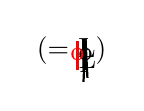
\begin{tikzpicture}[xscale=\myscalex-0.05,yscale=\myscaley-0.05]
\node (tone) at (3.5,0) {(= L)};
\node (syl) at (0,0) {\textsigma};
\node (syl2) at (2,0) {\red{\textsigma}};
\node (Rt) at (0,1) {o};
\node (H) at (-0.5,2) {L};
\node (R) at (0.5,3) {l};
\node (Rt2) at (2,1) {\red{o}};
\draw [thick] (syl.north) -- (Rt.south) ;
\draw [thick,red] (syl2.north) -- (Rt2.south) ;
\draw [thick] (Rt.north) -- (H.south) ;
\draw [thick] (Rt.north) -- (R.south) ;
\end{tikzpicture}
\end{minipage}
}

\newcommand{\OTLPolDef}{
\begin{minipage}{0.20\textwidth}
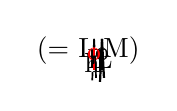
\begin{tikzpicture}[xscale=\myscalex-0.05,yscale=\myscaley-0.05]
\node (tone) at (3.5,0) {(= L.M)};
\node (syl) at (0,0) {\textsigma};
\node (syl2) at (2,0) {\red{\textsigma}};
\node (Rt) at (0,1) {o};
\node (H) at (-0.5,2) {L};
\node (R) at (0.5,3) {l};
\node (H2) at (1.5,2) {\epen{L}};
\node (R2) at (2.5,3) {\epen{h}};
\node (Rt2) at (2,1) {\red{o}};
\draw [thick] (syl.north) -- (Rt.south) ;
\draw [thick,red] (syl2.north) -- (Rt2.south) ;
\draw [thick] (Rt.north) -- (H.south) ;
\draw [thick] (Rt.north) -- (R.south) ;
\draw [semithick,dashed] (Rt2.north) -- (H2.south) ;
\draw [semithick,dashed] (Rt2.north) -- (R2.south) ;
\end{tikzpicture}
\end{minipage}
}

\newcommand{\OTLPolAlt}{
\begin{minipage}{0.20\textwidth}
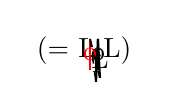
\begin{tikzpicture}[xscale=\myscalex-0.05,yscale=\myscaley-0.05]
\node (tone) at (3.5,0) {(= L.L)};
\node (syl) at (0,0) {\textsigma};
\node (syl2) at (2,0) {\red{\textsigma}};
\node (Rt) at (0,1) {o};
\node (H) at (-0.5,2) {L};
\node (R) at (0.5,3) {l};
\node (Rt2) at (2,1) {\red{o}};
\draw [thick] (syl.north) -- (Rt.south) ;
\draw [thick,red] (syl2.north) -- (Rt2.south) ;
\draw [thick] (Rt.north) -- (H.south) ;
\draw [thick] (Rt.north) -- (R.south) ;
\draw [semithick,dashed] (Rt2.north) -- (H.south) ;
\draw [semithick,dashed] (Rt2.north) -- (R.south) ;
\end{tikzpicture}
\end{minipage}
}

% Sec. 4.2, sixth tableau, polar questions with contour tones

\newcommand{\OTLLPolIn}{
\begin{minipage}{0.23\textwidth}
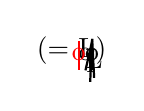
\begin{tikzpicture}[xscale=\myscalex-0.05,yscale=\myscaley-0.05]
\node (tone) at (5.2,0) {(= L)};
\node (syl) at (0,0) {\textsigma};
\node (syl3) at (3.4,0) {\red{\textsigma}};
\node (Rt) at (0,1) {o};
\node (Rt2) at (1.7,1) {o};
\node (Rt3) at (3.4,1) {\red{o}};
\node (H) at (-0.5,2) {L};
\node (R) at (0.5,3) {l};
\draw [thick] (syl.north) -- (Rt.south) ;
\draw [thick] (syl.north) -- (Rt2.south) ;
\draw [thick,red] (syl3.north) -- (Rt3.south) ;
\draw [thick] (Rt.north) -- (H.south) ;
\draw [thick] (Rt.north) -- (R.south) ;
\end{tikzpicture}
\end{minipage}
}

\newcommand{\OTLLPolDef}{
\begin{minipage}{0.23\textwidth}
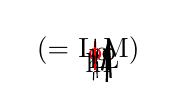
\begin{tikzpicture}[xscale=\myscalex-0.05,yscale=\myscaley-0.05]
\node (tone) at (5.2,0) {(= L.M)};
\node (syl) at (0,0) {\textsigma};
\node (syl3) at (3.4,0) {\red{\textsigma}};
\node (Rt) at (0,1) {o};
\node (Rt2) at (1.7,1) {o};
\node (Rt3) at (3.4,1) {\red{o}};
\node (H) at (-0.5,2) {L};
\node (R) at (0.5,3) {l};
\node (H3) at (2.9,2) {\epen{L}};
\node (R3) at (3.9,3) {\epen{h}};
\draw [thick] (syl.north) -- (Rt.south) ;
\draw [thick] (syl.north) -- (Rt2.south) ;
\draw [thick,red] (syl3.north) -- (Rt3.south) ;
\draw [thick] (Rt.north) -- (H.south) ;
\draw [thick] (Rt.north) -- (R.south) ;
\draw [dashed] (Rt3.north) -- (H3.south) ;
\draw [dashed] (Rt3.north) -- (R3.south) ;
\end{tikzpicture}
\end{minipage}
}

\newcommand{\OTLLPolSkip}{
\begin{minipage}{0.23\textwidth}
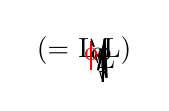
\begin{tikzpicture}[xscale=\myscalex-0.05,yscale=\myscaley-0.05]
\node (tone) at (5.2,0) {(= L.L)};
\node (syl) at (0,0) {\textsigma};
\node (syl3) at (3.4,0) {\red{\textsigma}};
\node (Rt) at (0,1) {o};
\node (Rt2) at (1.7,1) {o};
\node (Rt3) at (3.4,1) {\red{o}};
\node (H) at (-0.5,2) {L};
\node (R) at (0.5,3) {l};
\draw [thick] (syl.north) -- (Rt.south) ;
\draw [thick] (syl.north) -- (Rt2.south) ;
\draw [thick,red] (syl3.north) -- (Rt3.south) ;
\draw [thick] (Rt.north) -- (H.south) ;
\draw [thick] (Rt.north) -- (R.south) ;
\draw [dashed] (Rt3.north) -- (H.south) ;
\draw [dashed] (Rt3.north) -- (R.south) ;
\end{tikzpicture}
\end{minipage}
}  
  
\newcommand{\ilit}[1]{#1\il{#1}}    
\newcommand{\isit}[1]{#1\is{#1}}  

\makeatletter
\let\thetitle\@title
\let\theauthor\@author 
\makeatother

\newcommand{\togglepaper}[1][0]{ 
  \bibliography{../localbibliography}
  %% hyphenation points for line breaks
%% Normally, automatic hyphenation in LaTeX is very good
%% If a word is mis-hyphenated, add it to this file
%%
%% add information to TeX file before \begin{document} with:
%% %% hyphenation points for line breaks
%% Normally, automatic hyphenation in LaTeX is very good
%% If a word is mis-hyphenated, add it to this file
%%
%% add information to TeX file before \begin{document} with:
%% \include{localhyphenation}
\hyphenation{
affri-ca-te
affri-ca-tes
com-ple-ments
par-a-digm
Sha-ron
Kings-ton
phe-nom-e-non
Daul-ton
Abu-ba-ka-ri
Ngo-nya-ni
Clem-ents 
King-ston
Tru-cken-brodt
Tab-leau
cophono-logies
mark-edness
Ti-gri-nya
a-mong
Car-stens
Lu-bu-ku-su
}
\hyphenation{
affri-ca-te
affri-ca-tes
com-ple-ments
par-a-digm
Sha-ron
Kings-ton
phe-nom-e-non
Daul-ton
Abu-ba-ka-ri
Ngo-nya-ni
Clem-ents 
King-ston
Tru-cken-brodt
Tab-leau
cophono-logies
mark-edness
Ti-gri-nya
a-mong
Car-stens
Lu-bu-ku-su
}
  \papernote{\scriptsize\normalfont
    \theauthor.
    \thetitle. 
    To appear in: 
    Emily Clem,   Peter Jenks \& Hannah Sande.
    Theory and description in African Linguistics: Selected papers from the 47th Annual Conference on African Linguistics.
    Berlin: Language Science Press. [preliminary page numbering]
  }
  \pagenumbering{roman}
  \setcounter{chapter}{#1}
  \addtocounter{chapter}{-1}
}

\newcommand{\upstep}{\textupstep}


% \newcounter{tableauxcounter}

\renewcommand{\textltailn}{ɲ}
\renewcommand{\textbardotlessj}{ɟ}

\newcommand{\emphkh}[1]{\textit{#1}} %originally \textbf, banned by the guidelines



\definecolor{lsDOIGray}{cmyk}{0,0,0,0.45}


\newcommand{\xuparrow}[1]{%
  {\left\uparrow\vbox to #1{}\right.\kern-\nulldelimiterspace}
}
\renewcommand \textupstep[1]{\char"A71B#1}
\renewcommand \textdownstep[1]{\char"A71C#1}
 
 \newcommand{\ꜛ}{\textsf{ꜛ}}
 
\def\biberror{\undefined}


\newcommand{\OTbox}[1]{\resizebox{.88\textwidth}{!}{#1}}
 
\usepackage{pifont.sty}

\title{When Northern Swahili met southern Somali} 
\author{%
 Derek Nurse \affiliation{\ }
}
% \chapterDOI{} %will be filled in at production

% \epigram{}

\abstract{ Some twelve hundred years an incipient Northern Swahili community had moved up the Kenya coast as far as the Lamu Archipelago, where it came in contact with one or more Somali communities and the isolate Dahalo community. This paper initially uses phonological innovations in the early Swahili dialect to establish the general fact of contact, and then attempts to use sets of loanwords to identify the Somali source. Due to inadequate sources, it has proved difficult to identify the source(s) with certainty but initial contact with Tunni over some centuries, followed by later contact with Garre, is the most plausible explanation. The Tunni and Garre later exited, the latter leaving strong traces behind in Boni. }

\begin{document}

\maketitle


\section{Purpose}\label{sec:nurse:1} 

The target here is a micro-area in NE Kenya and SE Somalia.\footnote{The label “southern \ili{Somali}” is used in the title solely as a convenient geographical term. By contrast with Northern \ili{Swahili}, southern \ili{Somali} is not a recognized linguistic grouping.} It was once home to where northern \ili{Swahili} (including \ili{Mwiini}\footnote{\ili{Mwiini} is here considered a Northern \ili{Swahili} dialect, although others regard it as a separate language.}, the language of Brava) and some of its relatives are assumed to have emerged and developed, starting some 1200 BP, amidst a background of southern \ili{Somali} communities. This has been suggested before (\citealt{Nurse1983}; \citeyear{Nurse1985}) but not examined in such detail. The main differences here are the a) inclusion of \ili{Mwiini}, b) inclusion of southern \ili{Somali} (see the list in \sectref{sec:nurse:2}, below) other than \ili{Aweera} = \ili{Boni}, and c) stratigraphy of the Northern \ili{Swahili} Dialects (ND). The analysis involves the use of phonological innovations and \isi{lexical borrowing}, and includes some non-linguistic information.

\section{Players, in order of chronological entry on stage}\label{sec:nurse:2}

\subsection{Dahalo}\label{sec:nurse:2.1} 

\ili{Dahalo} is a \ili{Cushitic} language with a \ili{Khoesan} component (lexis, clicks) (see \figref{fig:nurse:1} for a map). \ili{Khoesan} split from \ili{Sandawe} at least 20,000 years ago (S. Tischkoff pc).\footnote{Dates are approximate. Populations from Ethnologue \citep{Lewis2015}.}  \ili{Khoesan} communities are assumed to have been spread across East Africa from Ethiopia south for many millennia. We do not know when or where \ili{Khoesan} and \ili{Cushitic} came together to form \ili{Dahalo}, nor how long the \ili{Dahalo} have been in situ, although minor hints suggest several millennia \citep{Nurse1986}. Today a few hundred (?) aging \ili{Dahalo} speakers remain. 

\begin{figure}
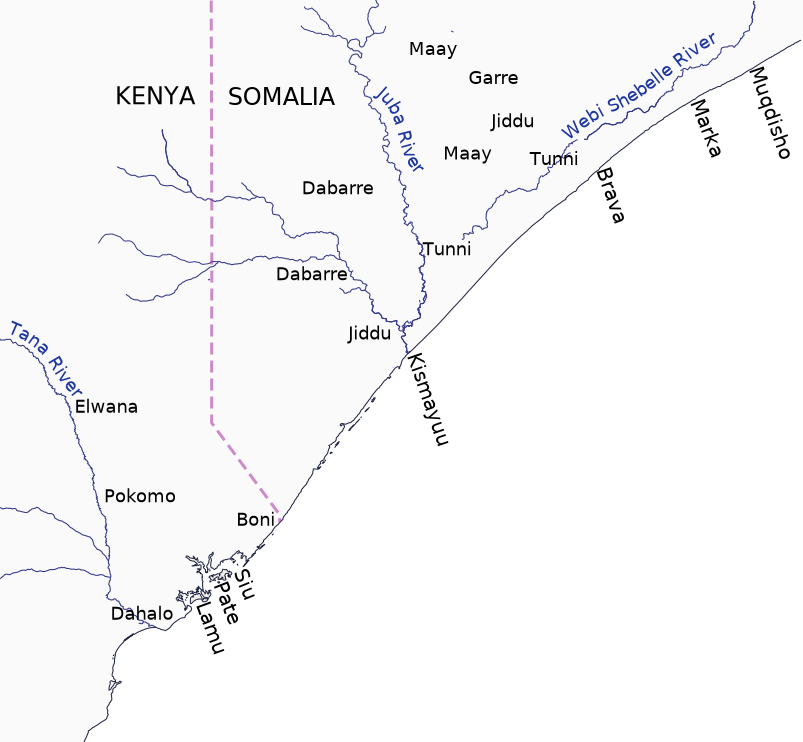
\includegraphics[width=\textwidth]{figures/nurse.pdf}
\caption{Linguistic communities in the Kenya-Somalia border area}
\label{fig:nurse:1}
\end{figure}

\subsection{Somali}\label{sec:nurse:2.2} 

Early Eastern Omo-Tana communities started to move SE into Somalia ca. 3000~BP and were in situ in southern Somalia by 2000 BP \citep{ehret1995}. Many local movements ensued over the next two millennia. Six \ili{Somali} dialect communities near the target area now can be assumed to have been so also in the past, and are the likely candidates as sources for the material in the ND. They are the:\footnote{The distribution of these southern \ili{Somali} communities is based on maps dawn by Lamberti in the 1980s \citep{Lamberti1983}, before civil war erupted in 1991. They may have changed in the meantime. The outbreak of war had other effects. Up to 1991 the language situation in \ili{Somali} was fairly stable but when the central government collapsed, coastal \ili{Swahili} communities were attacked, genocide followed, and the communities collapsed. Dialect ability in the ND communities in northern Kenya has been reduced by a combination of economic and educational factors.}

\begin{enumerate}
\item  \ili{Maay}, interriverine\footnote{“Interriverine” refers to the area along and between the rivers Juba and Shebelle, the only well watered part of the region and thus long a magnet for farmers and pastoralists.}, from just south of Muqdisho almost to Kismayu, with over 500,000 speakers

\item \ili{Tunni}, coastal, from near Merka to north of Kismayuu. 20,000 to 60,000 speakers. Earlier, possibly also further south. 

\item \ili{Dabarre}, interriverine. 20,000 to 50,000 speakers. \ili{Tunni} and \ili{Dabarre} are similar. \ili{Dabarre} is little known. 

\item \ili{Jiddu}, interriverine and coast south of Brava. 20,000 to 60,000 speakers. Not enough is known.

\item \ili{Garre}/\ili{Karre}\footnote{I follow Tosco and use \ili{Karre} for the language, \ili{Garre} for the/a clan. Also spelled “\ili{Karee}”.}, interriverine and widely scattered, with over 50,000 speakers.

\item \ili{Boni}, also called \ili{Aweera}. They live in a small area 60km long, mostly in NE Kenya with a few in SE Somalia, in villages in a forest bordering the coast. 3,000 speakers. \ili{Karre} and \ili{Boni} are similar. Along with \citet{Tosco1994} I assume that \ili{Boni} is a Dahaloised variety of \ili{Karre} that arose when the \ili{Karre} moved down to the coast into contact with \ili{Dahalo}.

\end{enumerate}

Other than the \ili{Boni} and the more recent \ili{Orma} and northern \ili{Somali}, no \ili{Somali} \ili{Cushitic} group is south of Kismayuu today, so some group or groups once in situ here, have migrated north (see \sectref{sec:nurse:6}). \citet{Ali1985} suggests that the \ili{Garre} did not withdraw north but were rather absorbed into the \ili{Orma} moving south. 

\subsection{Bantu}\label{sec:nurse:2.3} Early Bantu moved into East Africa in the closing centuries BC, and one group, labeled the North East Coast Bantu, had reached an area in NE Tanzania, bounded by Mombasa and the Usambara, Taita, and the Pare Mountains, by the early centuries AD. All relevant Bantu languages here form part of the Sabaki group, a subset of NECB\footnote{The Northeast Coast Bantu, a linguistic grouping involving  over 20 communities along the coast of southern Somalia, Kenya, and northeastern Tanzania. See, inter alia, \citealt{Nurse1993}: 4-19.}. The early ancestral Swahili northern dialect (ND) community moved up along the immediate hinterland of the Kenya coast from NE Tanzania and was most likely living in villages in northern Kenya, in the Lamu Archipelago and adjacent mainland coast, slightly before 800 AD. Two other early Sabaki communities, ancestral to Pokomo and Mijikenda, had by this time also spread into the interriverine area in southern Somalia. The early Elwana community was probably along the Tana River in NE Kenya \citep[485ff, 499ff]{Nurse1993}. The three earliest settlements on the Kenya coast are on Pate and Lamu Islands, at or slightly before 800 AD, with nearby sites on the mainland being slightly later \citep{Wilson2016}. The ND and related Sabaki communities are the: 

\begin{enumerate}

\item \ili{Mwiini} (ND), up to 1991 exclusively in and around Brava, 10,000 to 15,000 speakers, now scattered, worldwide, few still in Brava, new speakers said to be emerging as outsiders move in (Vianello, p.c).

\item \ili{Bajuni} (ND), SE \ili{Somali} and NE Kenya coast and islands. Few speakers are left in Somalia. Ca.\,20,000 Bajunis in NE Kenya, but how many are good speakers? 

\item \ili{Siu} (ND), in and around \ili{Siu} Town, northern \ili{Pate} Island. 6,000.

\item \ili{Pate} (ND), in and around \ili{Pate} Town, \ili{Pate} Island. 3,000.

\item \ili{Amu} (ND), in and around Lamu Town, Lamu Island. 15,000. Also other lects on Lamu Island.

\item \ili{Malindi} (ND), in and around \ili{Malindi} Town, between Lamu and \ili{Mombasa}. Size of population  speaking the dialect unknown.

\item \ili{Mombasa} (ND), \ili{Mombasa} city. It is likely that >25,000 speak the main dialect, Mvita. Also other smaller lects in and around around \ili{Mombasa}, mostly dead or dying.  \ili{Malindi} and \ili{Mombasa} are largely ignored in what follows.

\item \ili{Elwana}. Along Tana River, Bura to Garissa. >8,000.

\item \ili{Pokomo}. Along Tana River, from coast to Bura. >65,000.

\item \ili{Mijikenda}. Just inland of coast north of \ili{Mombasa}. >630,000.

\end{enumerate}

\subsection{Communities excluded from this study}\label{sec:nurse:2.4} 

Since the \isi{focus} here is from 800 to 1400 AD, besides the communities above four others known to have been in the area over the last two millennia played little or no role: (1) an unidentified \ili{Bantu} community in the interriverine area in the early centuries AD, (2) the \ili{Mushunguli}, along the Juba, descendants of escaped slaves from Tanzania, who settled there in the nineteenth century, (3) \ili{Orma}, and (4) Northern \ili{Somali}, who both arrived from the north over the last 500 years, too late to influence the events being discussed, although both are now present in the area. 

\section{Aim and assumptions}\label{sec:nurse:3} 

The purpose of this paper is twofold, to: see if this archaeology-based scenario can be linked to linguistic -- specifically phonological -- innovations within the ND, and to try link any such developments to a specific southern \ili{Somali} community. 

Northern \ili{Swahili} refers to the communities speaking \ili{Swahili} dialects from Brava down to the \ili{Mombasa} area and just south. The archaeological sites in the whole area, assumed to be \ili{Swahili}, were located in the Lamu Archipelago and{\slash}or adjacent mainland, slightly before 800 AD. I assume these to be those of the Proto-ND community. The northern communities at \ili{Mombasa} and maybe \ili{Malindi} and Mambrui must have been the first to move out of the area, as \ili{Mombasa} shows signs of \ili{Swahili} settlement already by the late 11\textsuperscript{th} century. They were followed closely by the ancestors of the \ili{Bravanese}, and maybe of people formerly beyond Brava at Munghia, Merka, Gezira, and Mkudisho\footnote{The name Shaangani, a Mkudisho quarter, and some pottery sherds there, suggest \ili{Swahili} connections.}, who had all moved north by ca 1100 AD. Archaeological sites in the traditional area occupied by \ili{Bajuni} are later, starting in the 14\textsuperscript{th} or 15\textsuperscript{th} century \citep[91]{Wilson1992}, along the 250km line from Dondo and adjacent settlements on the Kenya coast, north as far as Kismayu, That these dates are later maybe because archaeological data is incomplete or because the ancestors of the Bajunis spread along the coast later than the other communities. So far, this chronology is based largely on archaeology. The area in which the proto-ND communities lived was shared with one (or more?) southern \ili{Somali}-speaking communities. Other than the tiny and low-status \ili{Boni} community, no southern \ili{Somali} communities live in that area today. 

\section{Phonological innovations: ND dialects including Malindi and Mombasa}\label{sec:nurse:4} Southern Swahili dialects, from the Kenya/Tanzania border south, are conservative phonologically -- that is, they are close to their Sabaki and North East Coast Bantu forebears -- while all the northern dialects have innovated, so it is easier to arrange the latter stratigraphically as branches on a genealogical tree. Several dozen innovations\footnote{For instance, over 30 phonological features distinguish Bajuni from Standard Swahili (see \citealt{Nurse2013}/2011, click on \textit{Bajuni Database}, and go to the list at the end of \textit{Wordlist)}.}  are scattered across the ND spectrum, but most are local and recent, and/or cannot be clearly linked to Somali influence. Those in \tabref{tab:nurse:1} are significant because they occur in all ND and have diagnostic value because they do suggest a Somali source.

%%please move \begin{table} just above \begin{tabular
\begin{table}
\caption{Dentalization in Northern Swahili\footnote{Comments on the table. Underlining = dental, ny = palatal, c, j = alveopalatal. For \#6 I heard only [s] in Kenyan Bajuni in the 1970s, but have since heard [θ] from some Somali Bajunis. For \#7, Mwiini behaves inconsistently, some words having the dental, others the palatal, no obvious conditioning factors. My guess is that the dentals, or the process itself is a loan from Bajuni where dental nasals are the regular outcome and Bajuni was the nearest community to the south. What happens in \#8 might be a systemic compensation for \#1, which led to all ND having (inherited) /t/ and (innovated) /ṯ/ for a while – the subsequent affrication made the two less similar. Siu and Pate generally behave like Amu but here as Bajuni. I would guess that the change of [t] to [c] occurred under Bajuni influence. Portuguese records indicate that Bajuni influence and numbers were much greater in the past than today.}}
\label{tab:nurse:1}
\begin{tabularx}{\textwidth}{lCCCCCC}
\lsptoprule
 & \multicolumn{4}{c}{North ND} &  \multicolumn{2}{c}{South ND} \\
\midrule 
& \ili{Mwiini} & \ili{Bajuni} & \ili{Siu}/\ili{Pate} & \ili{Amu} & \ili{Malindi}, \ili{Mombasa} & Base form/SD\\
\midrule
&  &  &  &  &  & \\
1 & ṯ & ṯ & ṯ & ṯ & ṯ & [c]\\
2 & \uline{nd} & \uline{nd} & \uline{nd} & \uline{nd} & \uline{nd} & [nj]\\
3 & nd\textsuperscript{r} & nd\textsuperscript{r} & nd\textsuperscript{r} & nd\textsuperscript{r} & nd\textsuperscript{r} & [nd]\\

\tablevspace
4 & nz & \uline{nd} & \uline{nd} & \uline{nd} & nz & [nz]\\

\tablevspace
5 & z & ð & ð & z & z & [z]\\
6 & s & θ/s & s & s & s & [s]\\
7 & ny/ṉ & ṉ & ny & ny & ny & [ny]\\

\tablevspace
8 & t & c & c & t & t & [t]\\
\lspbottomrule
\end{tabularx}
\end{table}
These are arranged in approximate chronological order. Numbers 1, 2, 4, 5, 6, 7 involve some form of dentalization. Among coronals, worldwide \citep{Maddieson1984}, in Africa, and in East African \ili{Bantu}, alveolars are more common than dentals. All the \ili{Somali} dialects in the area (also \ili{Orma}) have a dental series as their only or predominant coronal set. Few have phonemic voiced fricatives, although most have [ð] as an allophone of a /d/. Thus it seems that by entering a \ili{Somali} “dental” area, early ND made an adaptive articulatory choice. \ili{Elwana}, \ili{Pokomo}, and \ili{Mijikenda} have also acquired dentality \citep[572-5]{Nurse1993}. Three different mechanisms are involved in the acquisition: 

\begin{enumerate}
	
\item the dentals enter in large sets of borrowed vocabulary, as in \ili{Pokomo} and \ili{Mijikenda};
\item inherited alveolars became dental, as in \ili{Elwana}, presumably by the community absorbing many outsiders for whom dentality was the norm; 
\item a phonetic process for the change from (pre)palatal to dental, as in the ND. In both cases the tongue lies in the same region but different parts of the tongue act alternately as the active articulators at the point where they lie. For palatals the blade operates on the palate, while the apex is raised, lying behind the teeth. For dentals, the apex operates on the teeth, while the blade is lowered from the palate. Disposition of blade and tip of tongue is identical or similar in both but, in a kind of rocking \isi{movement}, one part is raised as the other is lowered.   

\end{enumerate}


This is discussed in more detail in \citealt{Nurse1985}, the results are exemplified in \citet[572-575]{Nurse1993} and the details are not discussed further here. 

 It can be seen that \ili{Bajuni} is at the centre of the dentalization changes, being affected by all six innovations, \ili{Siu}/\ili{Pate} by four, \ili{Amu} by three, \ili{Mwiini} and the \ili{Mombasa} dialects by only two. \#3 and \#8 do not involve dentalization and are only mentioned or the sake of completeness. 

  What do \#1, 2, 4, 5, 6, and 7 tell us about the stratigraphy of the northern dialects? P-ND is defined by \#1, 2, 3, which developed presumably in one or more of the early settlements, from about 800 AD to before just 1100 AD, when early \ili{Mwiini} and \ili{Mombasa} broke away. \#4 developed while early \ili{Bajuni}, \ili{Amu}, \ili{Siu}, and \ili{Pate} were still adjacent and more or less in situ, between 1100 AD and when \ili{Bajuni} started to spread along the coast. The implementation of all six changes in \ili{Bajuni} suggests, by staying more or less in situ on the coast, it remained open to ongoing and later \ili{Somali} influence (\#5, 6, 7), after \ili{Mwiini} moved north, \ili{Mombasa} south, and \ili{Amu}/\ili{Siu}/\ili{Pate} stayed the islands. 

\section{Lexical borrowing from Somali in the ND dialects}\label{sec:nurse:5} The set of phonological innovations in \tabref{tab:nurse:1} point to pressure from Somali-speaking communities but do not identify specific communities. But which Somali? The most obvious way of identifying possible donor communities is by examining loan sets, first those common to all ND, which would point at borrowing in the 800 to 1100 AD period, then in Bajuni/Amu/Siu/Pate, the group left after Mwiini and Mombasa broke away, then in Mwiini, Bajuni, and Amu/Siu separately, and finally in other possible groupings.

\subsection{Sources}\label{sec:nurse:5.1} It is relevant to mention briefly the quality and quantity of the data available. For Dahalo (\citealt{Nurse1986}; \citealt{Ehret1989}; \citealt{Tosco1991}; various minor sources), Mwiini \citep{Kisseberth2004}, Bajuni, Amu, Siu, Pate (\citealt{Sacleux1939}; \citealt{Nurse2013}/2011), Tunni (\citealt{Tosco1997}; Vianello p.c.; Ehret's notes), Boni  (\citealt{Heine1977}; \citeyear{heine1982}; \citealt{sasse1979}), Karre \citep{Tosco1994}, Elwana (\citealt{nurse1994}; \citeyear{Nurse2000}), Giryama = Miji Kenda \citep{Deed1964}, Pokomo (various) reasonable data exists but only for Swahili dialects and Giryama/Mijikenda are the quantities of data really adequate. For other southern Somali dialects the lexical data is poor in quantity but also often in quality. 

  This is important because without large bodies of lexical data it is not possible to pinpoint the language donor communities properly.

\subsection{Karre and Boni: the devoicing of Somali morpheme initial /d/ and /g/, and the reduction of NC to C (stop)}\label{sec:nurse:5.2} Boni and Karre share features which distinguish them from other Somali varieties. One is the devoicing of Somali morpheme initial /d/ and /g/. So where other Somali varieties have \textit{daar} ‘touch’ and \textit{guur} ‘migrate, move house’, Karre and Boni have \textit{taar} and \textit{kuur}. P-Somali \textit{cimbir} ‘bid’ but G/B \textit{shim(m)ir}. In what follows I take the position that Boni is the result of a coming together of Karre and Dahalo or a Dahalo-like language, when the Karre moved into what is now the Boni area. The term “coming together” is used advisedly, as there are different explanations of how this took place.  

\subsection{The sociolinguistic picture}\label{sec:nurse:5.3} There are two relevant factors. One is the size of the communities involved. It can be seen from \figref{fig:nurse:1} that today the southern Somali communities (except Boni) are much larger than the ND communities. While it is tricky to guess at the size of earlier Somali communities, it is safe to say that the Swahili communities were always small, largely because they depended on wells for fresh water. The wells had and have a balance of fresh and salt water, and if too much fresh water is extracted, the well is eventually overwhelmed by salt water, becoming undrinkable, and the dependent community is doomed.\footnote{This happened at Ngumi Island, a Bajuni settlement in southern Somalia, while at nearby Chula Island, the water is only fit for cattle, and water has to be brought in for humans.}  So it is reasonable to guess that relatively small Swahili communities on the islands were surrounded by larger mainland Somali communities. In such a situation, the likely direction of borrowing – of language and other material – is from larger to smaller. 

  The second factor is economic. As early \ili{Sabaki} groups – early ND, \ili{Elwana}, \ili{Pokomo}, \ili{Mijikenda} -- moved up the coast, they almost certainly combined subsistence farming with hunting. At some point early \ili{Swahili} communities made the move to maritime activities (fishing, and trading across the Indian Ocean). \citet{Wilson2016} summarizes what was found by the archaeologists \linebreak(Chittick, Horton) who excavated the three earliest large sites on the island, \ili{Pate}, Shanga, Manda. At \ili{Pate}, fish, turtle, chickens, cattle, camels, wild ungulates were present in the deepest levels, 750--850 AD, and sheep/goats by 850--1000 AD. At Shanga, fish were early but only in quantity after 1000, and chickens also appear early. Sheep/goats and cattle are in the record by 840, but in quantity only after about 980. Local hunting groups, such as \ili{Dahalo}, on the adjacent mainland relied on hunting and fishing. \citet[132]{Wilson2016} cites Horton’s suggestion that “Shanga might have been a multicultural society from its foundation, including (non-\ili{Bantu}?) pastoralist elements”. Camel bones at Shanga are dated at 1075 AD, and camels certainly came south with Somalis, possibly along with cattle. \citet[72]{Nurse1985} cite a tradition among the \ili{Pate} people that “the origin of \ili{Pate} was a person from the mainland who was of the Sanye\footnote{Name for any local hunting group.} tribe”. Clearly the non-linguistic evidence suggests the early presence of \ili{Somali} and other groups.

\subsection{Somali loanwords in various ND groupings}\label{sec:nurse:5.4} The total number of clear loanwords in the ND is much larger than what appears in this section. In \tabref{tab:nurse:2} are included only the words which are loans in the ND and have a likely origin in some Somali dialect (or Dahalo, or maybe Orma).

%%TODO Idk how to make this fit. Two tables?
\begin{table}
\footnotesize
\caption{Somali loanwords shared by all ND = early ND}
\label{tab:nurse:2}
\begin{tabularx}{\textwidth}{>{\raggedright}p{2.75cm}>{\raggedright}p{1.5cm}p{1.2cm}Q}
\lsptoprule
\ili{Mwiini} & \ili{Bajuni} & \ili{Amu} etc & \ili{Cushitic}\footnotemark{}\\
\midrule
\textit{aabo} ‘a male name’ & \textit{abawa} ‘older brother’ & abawa & T \textit{abow/aboo}, B \textit{ab’ue’}, general S \textit{abboow(e)}, M \textit{aawow} ‘dad’. Is the Mw item from the same source as the others?\\
\textit{baaya}

‘my older sister’

\textit{bay and abbaay} ‘female names’,

\textit{abadhe} from T & \textit{abaya} ‘older sister’ & \textit{abaya} & General S \textit{abbaaye},

T \textit{abaaya  (abada} ‘title for women in poetry’), not in B\\
\textit{hawa’adi}  & \textit{avahadi} ‘gum for earache’ & \textit{avahadi} & prob. from T, as other S shapes are different\\
\textit{buru} ‘small fried wheat cake’ & \textit{buru} ‘maize’ & buru & B \textit{b’uuru} ‘maize’, \ili{Arabic} \textit{burr} ‘flour, wheat’, common S, \ili{Maay} ‘pie’, PSC \textit{bur}{}-, Dah \textit{b’uru.} From \ili{Arabic}?\\
\textit{dambari} ‘beestings’ & \textit{damari}\footnotemark{} & \textit{tamari} & S \textit{dambar,} d > t and mb > m characterize G and B. G \textit{tamar} Dah \textit{kamari} (k a mistake for t?)\footnotemark{}\\
\textit{daara} ‘touch’ & \textit{dara} & \textit{dara} & General S \textit{daar}, Bo \textit{taara}, \ili{Maay} taar\textbf{{}-} \\
\textit{dhaayika ‘}melt’ & \textit{dayuka} & \textit{dayuka, deyuka} & S/Tu dhay ‘spread ointment’\\
\textit{chi-d}\textit{uku} ‘navel’ & \textit{doko} ‘anus’ & \textit{doko} & S dhuuq \textit{‘vagina’}\\
\textit{dhu} ‘marrow’, & \textit{i-d}\textit{uhu} ‘marrow’ & \textit{duhu} & S dhuux, T ‘marrow’, M \textit{dhuu}\\
\textit{dhuko} ‘deaf’

dhaghaala ‘partly deaf’ & \textit{duko} ‘deaf’ & \textit{duko} & S \textit{dhegoole}, J \textit{dhagaali,} M dheghaal, PSC \textit{duux,} Dah. \textit{d’uuko.} So dhukay ‘ear wax’\\
\textit{duguwa} limp’ & \textit{dukuva} ‘be lame’ & \textit{dekua} & S \textit{dugua,} M \textit{dugh-ow} (note g to k in Baj, \ili{Amu} etc)\\
\textit{fuura ‘}swell’ & \textit{fura} & \textit{fura} & S, J, Dah all \textit{fuur}\\
\textit{i-garabu} ‘shoulder blade’ & \textit{i-garabu} & \textit{garabu} & S, T, M all \textit{garab}, J \textit{garaw,} (but G \textit{karab}, B \textit{karub})\\
\textit{guura} ‘move, migrate’ & \textit{gura} & \textit{gura} & S, T, etc \textit{guur (}G and B \textit{kuur)}\\
\textit{i-goroori} & \textit{i-gururu} ‘curdled milk’\textit{,  also kirori} & \textit{gururu} & S \textit{garoor}, M \textit{guruur}, T \textit{goroor,} \\
\textit{mazu  ‘}banana’ & \textit{idhu} & \textit{izu} & Common S, B \textit{maadu} (pl), Dah \textit{madhu}. From \ili{Arabic}?\\
\textit{chi-skit}\textit{a} ‘dried meat or fish’ & \textit{musikit}\textit{a} ‘strip of dried meat’ & \textit{musikit}\textit{a} & Dah \textit{sikkwit}\textit{a, misikit}\textit{a}\\
\textit{muna} ‘younger brother/sister’ & \textit{mnuna} & \textit{mnuna} & B \textit{bamuna} ‘younger sister’\\
\lspbottomrule
\end{tabularx}
\end{table}
\addtocounter{footnote}{-3}
\stepcounter{footnote}\footnotetext{B = Boni, Dab = Dabarre, Dah = Dahalo, G = Karre, J = Jiddu, M = Maay, PSC = Proto-Southern Cushitic (Ehret), S = Somali T = Tunni}
\stepcounter{footnote}\footnotetext{Is this a mistake for tamari?}
\stepcounter{footnote}\footnotetext{‘Beestings’ (first milk) and ‘limp’ are a puzzle: why does \ili{Mwiini} have the general \ili{Somali} shape in both while the other dialects have the \ili{Karre} shape? I assume separate borrowings.}

The strengths and weaknesses of this lexically based approach can be seen from this list (more items could be added). With the exception of ‘deaf’ and ‘dried meat’, all 20 items here are clearly from some \ili{Somali} source. They cannot be from \ili{Karre} or \ili{Boni} as they lack the devoicing of /d, g/, so we can say that they originate in D, J, M, or T. But beyond that, it is not possible to point at a clear single donor for these early ND borrowings: the available lexica do not show these items, so unambiguous source identification is impossible. The best candidate is \ili{Tunni}. For geographical and (sketchy) historical reasons, \ili{Maay} and \ili{Jiddu} are unlikely candidates. We do not know enough of \ili{Dabarre}. 

  I think it would be risky to draw too many conclusions about the nature of these loans until we have more complete data. However, most of these terms do not seem to indicate much economic or cultural influence from the \ili{Somali} contact, which suggests that \ili{Somali} influence may have resulted from sheer numbers. 

  At the breakup of the protocommunity, the earliest \ili{Bravanese} moved up north around 1100 AD, to Brava and maybe further (see \sectref{sec:nurse:3}). For their language, \ili{Mwiini}, there is a fine dictionary \citep{Kisseberth2004}, with some 5000 entries. Some entries are followed by a \ili{Swahili} form, so mostly of \ili{Bantu} origin, some are \ili{Arabic}, some are followed by a \ili{Somali} word, indicating probable \ili{Somali} origin, and some are followed by no reference to any other language. Some pages have not a single \ili{Bantu} entry. The authors admit they only consulted a Standard \ili{Somali} dictionary and had little access to material from \ili{Somali} dialects. Vianello (p.c.) has calculated that “some 20\% of the general lexicon consists of borrowings from \ili{Somali} and of \ili{Arabic} words that have entered \ili{Chimiini} through \ili{Somali}”. Standard \ili{Somali} is of northern origin but much of the material in \ili{Mwiini} is of southern or unidentified \ili{Somali} origin. The result is that the dictionary has many items not of \ili{Bantu}, not of \ili{Arabic}, and not of Northern/Standard \ili{Somali} origin. Thus the percentage of words of \ili{Somali} origin is likely to be much higher. My guess is it might be as high as 30\% or maybe 40\%. So many centuries of coexistence and bilingualism have resulted in very heavy borrowing in \ili{Mwiini} from \ili{Somali}. These items cannot be from \ili{Karre}/\ili{Boni} because they do not show the phonological characteristics of those dialects. Phonologically they might be from \ili{Tunni}, \ili{Dabarre}, Jiddi, or \ili{Maay}: it would be worthwhile identifying the phonological and lexical differences between these four and against the unidentified lexical items in \ili{Mwiini}. 

  \ili{Mwiini} has also been influenced in non-lexical (morphological, syntactic) ways. Some of these are discussed in \citet{nurse1991}, \citet{Henderson2010}, and \citet{Vianello2015}. 

From what we know of the history of Brava in recent centuries, the most likely source is \ili{Tunni}. They live and have lived in and around the town for centuries or maybe longer. Vianello (p.c) quotes a letter, written by influential \ili{Tunni} elders to the \ili{Italian} authorities in 1953, stating that they had been in the Brava region for 800 years, which of course cannot be confirmed. 

  After the departure of the \ili{Bravanese} to the north and Mombasans to the south, a rump of early \ili{Bajuni}/\ili{Amu}/\ili{Siu}/\ili{Pate} speakers remained.  A set of some 25 items is shared by those dialects.\footnote{For reasons of space, these and others following are not shown. I can send them to interested readers.}  They are a mixed bunch: some from an unidentified \ili{Somali} dialect (not G or B), a couple from \ili{Karre}/\ili{Boni} (‘beestings’, ‘limp’, see \tabref{tab:nurse:2}), some of unknown origin. It stands to reason that one of the sources might be the continuing presence of the same \ili{Somali} community that left its imprint on the original ND community (\tabref{tab:nurse:2}, \ili{Tunni}?).

  Next, the \ili{Bajuni} community spread north along the coast. \ili{Bajuni} has some 30 borrowings, many of which seem to be of \ili{Somali} origin. Contrary to expectation, few are unambiguously from \ili{Boni}/\ili{Karre}, but an interesting item is \textit{k\textsuperscript{h}}\textit{amasi} ‘clan’, with characteristic \ili{Boni}/\ili{Karre} devoicing, where \ili{Tunni} has \textit{gamaasi.}\footnote{There is another interesting possibility. In older \ili{Bajuni} poetry I found \textit{loya} ‘cattle’. Tosco (p.c) tells me he finds as the plural of \textit{lo’} in \ili{Karre} the form \textit{looyi}, which with the suffixed article gives \textit{looya} (vowel shortened to \ili{Bajuni} \textit{loya}) ‘the cows/cattle’. He describes ut as a “strong connection with \ili{Karre}’.} The exact \ili{Somali} source of most is again unclear but may be (?) one of the sources already mentioned (\ili{Tunni}). A few apparently originated in \ili{Dahalo}.\footnote{Sands finds it surprising that the \ili{Dahalo} could have had much impact. The main source of data for lexicon for flora and fauna in the ND was \citet{Sacleux1939}, a huge volume of 1000 pages of fine print. I started through it but was daunted and abandoned the task. Once all the data there has been extracted and compared with that for \ili{Dahalo} we will gain a better overview of the role of \ili{Dahalo}.} Ehret has pointed out to me that there is some evidence for a possible second \ili{Somali} group in far northeastern Kenya before 1500 AD. 

  After the \ili{Bajuni} exit, the \ili{Amu}, \ili{Pate}, and \ili{Siu} communities remained in situ. They share a small set of loans, but so small as to make conclusions impossible. Likewise, \ili{Mwiini} and \ili{Bajuni}, historically close geographically, share a small loan set from \ili{Somali}, but examination of these adds little to the general picture. They do not appear to be of \ili{Karre}/\ili{Boni} origin so may also be from \ili{Tunni}. 

\subsection{Conclusions from loanwords (and phonology)}\label{sec:nurse:5.5} There has been a continuous Somali-speaking presence on the mainland adjacent to the Lamu Archipelago from 800 AD – and probably much earlier – to the present. But the nature of the Somali presence changed during that period. For much of that time, except recently, speakers of southern Somali dialects probably outnumbered the ND communities. At a more recent point in the period the Karre appeared, then withdrew, leaving their imprint in place in the form of the Boni and their language. In the early part of the period – and continuing till an undefined date -- the Somali community was different – Tunni, Dabarre, Maay,\footnote{There are few serious suggestions that Maay played a role. It is included because it is in the area.}  or Jiddu. There may even have been more than one Somali presence, but it is more economical to assume a single community, unless more than one can be demonstrated. The most likely single candidate is the Tunni, until and unless more lexical data becomes available for the other communities (Dabarre, Maay, Jiddu). I had hoped to be able to show a better, more concrete conclusion.

The somewhat sparse evidence also suggests a \ili{Dahalo} presence in the area from the earliest period. Various articles in the bibliography deal with \ili{Dahalo} influence on individual non-\ili{Dahalo} language in the area but the picture would be improved by an examination of the phonological and lexical influence of \ili{Dahalo} across the whole area.\footnote{Some of the consonant changes listed by \citet[115-26]{Ehret1980}, or their outcomes, are similar to those undergone by other languages in the area.}  

\subsection{General non-linguistic history of the area} Several historians and others have weighed in on the (non-linguistic) history of the target area, and mainly on two topics: one, which was the original southern \ili{Somali} group that influenced early ND from 800 AD for several centuries, and two, when did the \ili{Garre} move south into the area.

The only substantial relevant claim about the original southern \ili{Somali} group is in \citet[15ff]{Lewis1969}. Following earlier \ili{Italian} scholars, who in turn had gleaned their information from \ili{Tunni} oral traditions, he states that \begin{quotation}“the \ili{Tunni} once lived on the Juba River, then moved south and settled between Kismayuu and Lamu in the tenth or eleventh centuries AD, then “later” moved north again, across the Juba to settle near Brava, where they live today (which is just north of Kismayuu to just south of Merka, including Brava).”\end{quotation} That is an amazing claim, as it is not based on language. The place and the date correspond quite closely to what is claimed above, on linguistic grounds. The starting point, the “tenth century”, corresponds quite closely to the 800 AD date suggested above. It contains an obvious flaw – what exactly is that dating based on? The linguistic picture needs to be firmed up by examining more closely these lexical borrowings in the ND and how they fit with \ili{Tunni}. We also need to know better when the \ili{Tunni} finally withdrew.

All sources agree that \ili{Garre} people moved south into the area: \ili{Bajuni} traditions are quite detailed on this – \ili{Garre} moved onto the islands from the north, original inhabitants e.g.\ on the north of Koyama Island were forced south, the newcomers carved their mark on a tree opposite Koyama Island before crossing over, \ili{Bajuni} clan names are of two kinds, one of \ili{Bantu} origin/topopnyms while the others are southern \ili{Somali} in origin, and one clan is even called the \ili{Garre} (the others have not been identified yet). The \ili{Garre} interacted with original hunter-gatherers, probably \ili{Dahalo}, resulting in the \ili{Boni} dialect, left behind when the \ili{Garre} withdrew or were assimilated into the \ili{Orma}.  

The point of disagreement concerns when the \ili{Garre} arrived. Some scholars have them arriving recently, just before 1700 AD, as the \ili{Portuguese} were leaving. At the other end of the scale, others, for example, \citet{Ali1985}, date the \ili{Garre} arrival seven centuries earlier, late in the first millennium AD. The loanword evidence in \sectref{sec:nurse:5.4} above, first in the rump language/dialects left after the departure of the \ili{Bravanese} and Mombasans and continuing through to the emergence of \ili{Bajuni}, suggest contact with \ili{Karre} starting some time after 1100 AD, thus inclining to the earlier date.

\section{A corollary: the southern dialects of Swahili}\label{sec:nurse:6} \citet[map p.345]{Möhlig1984} and \citet[map p.60]{Nurse1985}, independently, show the ancestors of the southern Swahili dialect (SD) communities, including Mwani in Mozambique, as migrating south from a Proto-Swahili origin in the Lamu Archipelago area. In view of the conclusions drawn here, that seems unlikely. All the Sabaki languages which originally went north to the Lamu area or further, show clear signs of Somali influence, phonological (esp. dentalization) and lexical. The SD show no such signs, for which there are two explanations. Either – less likely – the early SD community did go north but stayed a short time, short enough to have avoided all influence from Somali dialects, or – more likely – the SD never went north, having split from the ND at some prior point, which would mean that the Proto-Swahili community was located somewhere other than the Lamu area, somewhere further south. Where might the earliest SD have been located? Archaeology suggests the island of Kilwa, the earliest and largest site in the SD area, roughly contemporary at 800 AD with the three large early ND sites. And in that case, where might the putative Proto-Swahili area have been?

\section{Conclusion}\label{sec:nurse:7}  In the twelve centuries since this narrative began, huge changes have occurred in and around the target area. In 700 AD, only one southern Somali community, possibly Tunni, and the Dahalo lived there. Around 800 AD an early ND community arrived, along other Sabaki communities. The interaction between early ND and the Somali community changed early ND speech. Eventually that early Somali community withdrew – when? – and the Garre entered the scene. They interacted with Dahalo, resulting in the Boni dialect. Dahalo has declined slowly and inexorably over the whole period. First the Orma, then northern Somali moved steadily south into the area. The ND communities, who once lived on the islands and farmed extensively on the adjacent mainland, increasingly withdrew to the islands. This pressure from the north intensified, squeezing Orma into Kenya, followed by northern Somalis themselves, and pushing southern Somali communities south and east. For the ND, the final act came after 1991, when central government collapsed in Somalia, and the two remaining Bantu communities in Somalia, Bravanese and Bajuni, were reduced to almost zero as northern Somalis spread east and south. Since 1991, civil war has changed the linguistic picture to an as yet undetermined extent. 

\section{Acknowledgements} My thanks are due to Alessandra Vianello, Bonny Sands, Mauro Tosco, Tom Spear, Chris Ehret, Sarah Tishkoff, and Kirk Miller, for help with data, ideas, and corrections, and also to the two reviewers.

%Edwin: biblio entries added except Roma
\begin{comment}
\begin{verbatim}

Comfort, J. and  M, Paster. 2009. Notes on Lower Jubba \ili{Maay}. In Selected Proceedings of ACAL 38: Linguistic theory and African language documentation. ed. M. Matondo, F. McLaughlin, E.  Potsdam. Somerville, MA: Cascadilla Proceedings Project. 204-216. http://www.lingref.com/cpp/acal/38/index.html

Ehret, C. 1995. The Eastern Horn of Africa, 1000 BC to 1400 AD:~ The historical roots. In  A.J. Ahmed (ed.), The invention of Somalia. Lawrenceville, NJ:~ The Red Sea Press, 233-262.

Ehret, C. 2013. The extinct \ili{Khoesan} languages of Eastern Africa. In R. Vossen (ed). The \ili{Khoesan} languages. Abingdon: Routledge. 465-479.

Ehret, C., and  Ali, M.N. 1984. Soomaali classification. In Labahn, T. (ed.). Proceedings of the second Intl. conference of \ili{Somali} studies (Hamburg, August 1-6, 1983). Vol. 1: Linguistics and literature. Hamburg. Helmut Buske. 201-269.

Ehret, C. 1978. The SAM languages: A history of Rendille, \ili{Boni}, and \ili{Somali}. Afroasiatic Linguistics:   1-93.

Maddieson, Ian. Ladefoged. P, Sands, B. 1999. Clicks in East African languages. African Mosaic: Festschrift for J.A. Louw. ed. Rosalie Finlayson. Pretoria: University of South Africa, UNISA Press. 59-91.

Mumin, Meikal and  G.J. Dimmendaal. Forthcoming. Chimini. In Bostoen, K, D. Nurse, G. Philippson, Van der Velde (eds.), The \ili{Bantu} languages. 2\textsuperscriptnd edition. London: Routledge.

Nurse, D. 1982. The \ili{Swahili} dialects of Somalia and the Northern Kenya Coast, in M-F. Rombi (ed). Etudes sur le \ili{Bantu} Oriental. Paris: LACITO/CNRS. 73-146.

Nurse, D. 1991. Language contact, creolization, and genetic linguistics: The case of \ili{Mwiini}. In Proceedings of the Berkeley Linguistic Society 17, Special Session on African Language Structures. UC Berkeley. 177-187.

Nurse, D. 1992 Shungwaya and the \ili{Bantu} of Somalia: Some linguistic evidence. In H. M. Adams and  C.L. Geshekter (eds.). Proceedings of the First International Congress of \ili{Somali} Studies (1980). Chico CA. Scholars Press. 54-61.

Nurse, D. 1994 South meets North: Ilwana = \ili{Bantu} + \ili{Cushitic} on Kenya's Tana River. In P. Bakker and  M. Mous (eds.), Mixed languages. 15 Case Studies. Amsterdam. Instituut voor Functioneel Onderzoel van Taal en Taalgebruik. 215-224.

Nurse, D. 2010 The decline of \ili{Bantu} in Somalia. In F. Floricic (ed.), Essais de typologie et de linguistique générale, Mélanges offerts à Denis Creissels. Lyon : ENS Editions, 187-200.

Nurse, D. and  T. Spear. 1985. The \ili{Swahili}: reconstructing the history and language of an African society, 800-1500. Philadelphia: University of Pennsylvania Press.

Sasse, H-J. 1979. Entlehnung morphophonemischer Regeln im \ili{Boni}. Sprache und Geschichte in Afrika:   93-108.

Tonelli, L. 1999. The \ili{Karre} of Somalia: A sketch of its linguistic features. Afroasiatica  Tergestina: Papers from the 9th \ili{Italian} Meeting of \ili{Afro-Asiatic} (Hamito-Semitic) Linguistics, Trieste, April 23-24, 1998/Contributi presentati al 9º Incontro di Linguistica Afroasiatica (Camito-Semitica), Trieste, 23-24 \citealtApril1998. eds. Lamberti, M. and  L. Tonelli. Padova: Unipress. 373-379.

Roma: Ministero degli Affari Esteri, Direzione Generale per la Cooperazione allo Sviluppo, Comitato Tecnico Linguistico per l'Università Nazionale Somala.   (\urlhttp://host.uniroma3.it/centri/CentroStudi\ili{Somali}/ie_ar_testi.php)

Tosco, M. 2005. \ili{Karre}. Encyclopedia Aethiopica. Vol. 2. Wiesbaden: Harrassowitz. 709-710.

Iribemwangi, P (eds.), The Harmonization and Standardization of Kenya Languages,     Capetown: Centre for Advanced Studies of African Society. 263-280.


\end{verbatim}
\end{comment}

\sloppy
\printbibliography[heading=subbibliography,notkeyword=this]

\end{document}